% =============================================================================
% Materials and Methods — UAP report analysis pipeline (UFOSINT / UAP Foundry)
% -----------------------------------------------------------------------------
% Standalone-compilable methodology section. Every parameter, threshold and
% count in this document is taken from the implemented pipeline (uap_analyzer.py,
% scu_normalizer.py, api/services/*) and from measured runs, not from intent.
% Compile:  pdflatex methodology.tex  (twice, for references)
% =============================================================================
\documentclass[11pt,a4paper]{article}

\usepackage[utf8]{inputenc}
\usepackage[T1]{fontenc}
\usepackage[margin=2.5cm]{geometry}
\usepackage{amsmath,amssymb}
\usepackage{booktabs}
\usepackage{graphicx}
\usepackage{tikz}
\usetikzlibrary{arrows.meta,positioning,shapes.geometric}
\usepackage[hidelinks]{hyperref}
\usepackage{microtype}

\newcommand{\pkg}[1]{\texttt{#1}}
\newcommand{\field}[1]{\texttt{#1}}

\title{Materials and Methods:\\ A Statistical Analysis Pipeline for LLM-Structured UAP Report Corpora}
\author{Sinan Robillard}
\date{\today}

\begin{document}
\maketitle

\section{Materials and Methods}

\subsection{Overview and analytical framing}

The pipeline described here converts free-text unidentified anomalous phenomena (UAP)
reports into a structured, schema-conformant dataset and subjects it to categorical
association screening, conditional-independence testing, supervised feature-importance
analysis, and unsupervised text clustering (Figure~\ref{fig:pipeline}). The design goal
throughout is \emph{hypothesis generation under honest uncertainty}: the corpus is
observational and curated, the feature extraction is itself a measurement instrument
with quantifiable error, and every downstream statistic is therefore reported with the
safeguards appropriate to exploratory screening---bias-corrected effect sizes, bootstrap
confidence intervals, multiple-comparison control, sparsity diagnostics, and
cross-validated rather than single-split model evaluation. No output of this pipeline is
interpreted causally, and associations that survive screening are treated as candidate
hypotheses for confirmation on independent data rather than as findings.

\begin{figure}[htbp]
\centering
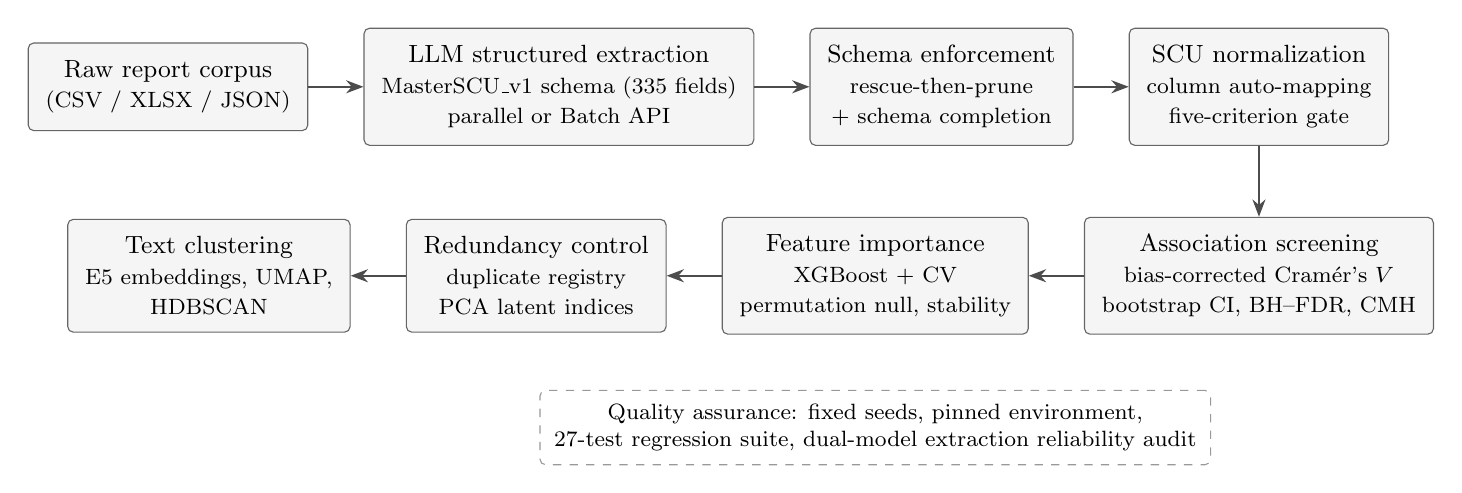
\begin{tikzpicture}[
  node distance=5mm and 7mm,
  stage/.style={rectangle, rounded corners=2pt, draw=black!60, fill=black!4,
                align=center, minimum height=9mm, inner sep=2.2mm, font=\small},
  qa/.style={rectangle, rounded corners=2pt, draw=black!40, dashed, fill=white,
             align=center, inner sep=1.8mm, font=\footnotesize},
  arr/.style={-{Stealth[length=2.2mm]}, thick, black!70}
]
\node[stage] (raw)   {Raw report corpus\\ \footnotesize (CSV / XLSX / JSON)};
\node[stage, right=of raw] (llm)  {LLM structured extraction\\ \footnotesize MasterSCU\_v1 schema (335 fields)\\ \footnotesize parallel or Batch API};
\node[stage, right=of llm] (post) {Schema enforcement\\ \footnotesize rescue-then-prune\\ \footnotesize + schema completion};
\node[stage, right=of post] (scu) {SCU normalization\\ \footnotesize column auto-mapping\\ \footnotesize five-criterion gate};
\node[stage, below=9mm of scu] (assoc) {Association screening\\ \footnotesize bias-corrected Cram\'er's $V$\\ \footnotesize bootstrap CI, BH--FDR, CMH};
\node[stage, left=of assoc] (xgb) {Feature importance\\ \footnotesize XGBoost + CV\\ \footnotesize permutation null, stability};
\node[stage, left=of xgb] (pca) {Redundancy control\\ \footnotesize duplicate registry\\ \footnotesize PCA latent indices};
\node[stage, left=of pca] (clus) {Text clustering\\ \footnotesize E5 embeddings, UMAP,\\ \footnotesize HDBSCAN};
\node[qa, below=7mm of xgb] (qabox) {Quality assurance: fixed seeds, pinned environment,\\ 27-test regression suite, dual-model extraction reliability audit};
\draw[arr] (raw) -- (llm);
\draw[arr] (llm) -- (post);
\draw[arr] (post) -- (scu);
\draw[arr] (scu) -- (assoc);
\draw[arr] (assoc) -- (xgb);
\draw[arr] (xgb) -- (pca);
\draw[arr] (pca) -- (clus);
\end{tikzpicture}
\caption{Analysis pipeline. Free-text reports are converted to a 335-field structured
schema by a large language model, repaired and completed against the schema, normalized
through the SCU eligibility gate, and analysed by complementary statistical and
machine-learning modules. Dashed box: cross-cutting quality-assurance measures.}
\label{fig:pipeline}
\end{figure}

\subsection{Data sources and extraction schema}

Source material consists of textual UAP/UAS incident reports assembled from public
archives (e.g.\ United States Air Force Project Blue Book records, FAA unmanned-aircraft
incident summaries, and curated civilian catalogues), ingested as CSV, XLSX, or JSON.
For each report, the free-text narrative and any selected auxiliary columns are
concatenated into a single extraction input; auxiliary source columns designated as
``carry-through'' (e.g.\ an authoritative date column) bypass extraction and are
re-attached to the structured output by exact alignment on the input text.

Extraction targets the \emph{MasterSCU\_v1} schema, a canonical master template of
335 leaf fields organised in 23 top-level blocks (record and study provenance, source,
date--time, location, witness, detection, object characteristics, behaviour and
kinematic performance, anomaly roll-ups, engagement types and flags, military context,
physical and physiological effects, entities, contact, environment, evidence,
classification, assessment, scenario codings, investigation, narrative, and context).
The schema is stored as a single JSON source of truth and embedded in every extraction
request. A hard output constraint is imposed on the ten engagement-type fields: exactly
one field must carry the primary code \texttt{P}, any number may carry the secondary
code \texttt{S}, and all others must remain blank.

\subsection{LLM feature extraction}

\subsubsection{Inference regimes}
Two interchangeable inference regimes are supported. In the \emph{parallel} regime,
requests are issued concurrently (default 10 worker threads) with JSON-mode decoding
and per-request retry under exponential backoff (initial wait 5\,s, doubling to a
600\,s ceiling, at most 10 attempts). Transient failures (HTTP~429 rate limits and
5xx server errors) are retried; permanent failures---exhausted quota
(\texttt{insufficient\_quota}), invalid credentials, or billing errors---trip a
process-wide circuit breaker that aborts the entire run on first occurrence, preventing
a pathological regime in which every queued report would otherwise retry a doomed call
(up to $10 \times 10 \times N$ requests). Completed responses are checkpointed to disk
after every request, making interrupted runs resumable without repeated cost.

In the \emph{batch} regime (OpenAI Batch API), requests are serialised to JSONL and
split into multiple jobs under two simultaneous caps: 50{,}000 requests per job and a
190\,MiB input-file limit (safety margin below the service's 200\,MiB ceiling, which
is otherwise exceeded because the full schema template is embedded in every request
line; a 9{,}565-report corpus produces $\approx$405\,MiB of request lines and is split
into three jobs). Request identifiers are global row indices, so multi-job outputs
reassemble deterministically, and result files downloaded out-of-band can be re-imported
and re-keyed to the original input texts.

\subsubsection{Schema enforcement: completion and rescue-then-prune}
JSON-mode decoding guarantees syntactic validity but not schema conformance, and two
systematic deviations were observed empirically. First, models omit keys they never
assign, despite instructions to emit blanks; because tabularisation unions keys across
records, a key omitted from every record silently deletes the column. Second, models
occasionally mis-nest structure: in one audited run a single response embedded eleven
top-level schema blocks inside the \field{military} object (creating 146 spurious
columns), and other responses transplanted assessment fields into the classification
block or invented fields drawn from prior knowledge of classification systems.

Both deviations are repaired deterministically at parse time, before any tabularisation
or joining with source columns. A \emph{rescue-then-prune} pass relocates each
non-blank off-schema value to its canonical path when that path is recoverable---by
longest path-suffix match (e.g.\ \field{military.investigation.timeliness}
$\rightarrow$ \field{investigation.timeliness}) or by unique leaf name (e.g.\
\field{classification.trustScore} $\rightarrow$ \field{assessment.trustScore})---with
the invariant that an existing value at the canonical path is never overwritten;
unrescuable keys (inventions and ambiguous leaves) are dropped and logged.
A \emph{schema-completion} pass then pads every record to the full template, so that
absent fields appear as explicit blanks rather than missing columns. In a retrospective
application to an affected corpus, this procedure relocated 112 misplaced values and
discarded 5 unrescuable cells, leaving zero off-schema columns.

\subsubsection{Extraction reliability across models}
Because the extractor is a measurement instrument, inter-model reliability was audited
by parsing the same corpus (a 60-report FAA unmanned-aircraft incident sample)
independently with two models (\texttt{gpt-4o-mini} and a DeepSeek chat model) and
aligning outputs by greedy token-Jaccard matching of narratives (threshold 0.55;
54 pairs matched at mean similarity $\approx$1.0). Agreement on both-filled values was
near-perfect for factual fields (year, month, state, country 96--100\%; city 98\%;
colour 95\%; witness count 88\%) and substantially lower for judgment fields
(day/night 69\%, primary shape 65\%, contradicts-UAP flag 58\%, explanation category
46\%, primary engagement type 54\%, Hynek classification 19\%). Fields with
below-70\% inter-model agreement are treated as model-dependent measurements and are
not used to support substantive conclusions without adjudication. Extracted
latitude/longitude values are treated as inferred geocoding rather than extraction and
are excluded from spatial inference.

\subsection{SCU normalization and eligibility gate}

Structured records are canonicalised by a deterministic normalizer: country and
U.S.-state names are mapped to ISO codes, location types, craft shapes and size bands
are mapped to controlled vocabularies, witness roles are tokenised and canonicalised,
and flag fields are upper-cased. The normalizer then derives the Scientific Coalition
for UAP Studies (SCU) five-criterion eligibility gate as boolean columns: (i) event
within the 1945--1975 study window; (ii) core fields present (complete date and
country); (iii) report received through an investigation channel; (iv) at least one
credible witness class (e.g.\ pilot, military, police, scientist); and (v) anomalous
characterisation, together with an engagement signal defined as at least one of nine
engagement-type fields coded \texttt{P} or \texttt{S}. Auxiliary resolvers (day/night
resolved; military-versus-public origin known) are computed alongside, and the
conjunction yields \field{scu\_eligible} with a per-criterion funnel.

Because extraction schemas evolve, the normalizer does not assume fixed column names.
An input-column resolver maps every canonical gate input onto the actual dataset
columns through a deterministic cascade---exact name, curated alias (e.g.\
\field{craft.size} $\leftarrow$ \field{object.size}; \field{investigation.source}
$\leftarrow$ \field{source.name}), unique path suffix, unique leaf name, and finally
fuzzy string similarity (Gestalt pattern matching, acceptance threshold 0.80)---with
every resolution, its method, and its confidence recorded in the audit and exposed for
manual per-field override in both user interfaces. Exact matches always take precedence
over aliases, preserving backward compatibility with legacy schemas. This mapping layer
was introduced after an audit showed that path re-parenting in MasterSCU\_v1 silently
starved three of the five gate criteria of data under exact-name matching.

\subsection{Missing data}

Missingness is first made explicit: a canonical \texttt{(missing)} level absorbs all
null encodings so that missingness is never fragmented across representations.
For exploratory completion, an optional model-based imputation trains one gradient-boosted
classifier per column on the rows where that column is observed (the \texttt{(missing)}
level is never a prediction target) and predicts the missing cells, either as the
maximum-probability class (single imputation) or by drawing $M$ samples per cell from
the predicted class distribution (multiple imputation), in which case the modal draw is
imputed and the per-cell agreement fraction is retained as a cell-level uncertainty.
Every imputed cell is displayed with the accuracy of its generating model (holdout and
cross-validated), visually distinguished from observed data, and imputed values are
excluded from inferential statistics: the imputation assumes missingness at random given
the observed fields, an assumption that is likely violated in curated UAP archives where
missingness can be informative (missing not at random), and single-imputation fills are
therefore treated as exploratory annotations only. Where imputation-based quantities are
carried into estimation, pooling across the $M$ completed datasets by Rubin's rules is
the prescribed procedure \cite{rubin1987}.

\subsection{Categorical association analysis}

\subsubsection{Effect size}
Pairwise association between categorical fields is quantified by the bias-corrected
Cram\'er's $V$ \cite{cramer1946,bergsma2013}. For an $r \times k$ contingency table with
$n$ observations and Pearson statistic $\chi^2$,
\begin{equation}
\tilde{\varphi}^2 = \max\!\left(0,\; \frac{\chi^2}{n} - \frac{(k-1)(r-1)}{n-1}\right),
\qquad
\tilde{V} = \sqrt{\frac{\tilde{\varphi}^2}{\min(\tilde{k}-1,\; \tilde{r}-1)}},
\end{equation}
with $\tilde{r} = r - (r-1)^2/(n-1)$ and $\tilde{k} = k - (k-1)^2/(n-1)$; degenerate
denominators return $V = 0$. Columns are screened by cardinality (binary, low
$\le 9$, and medium $< 30$ levels are eligible; constant and high-cardinality
free-text columns are excluded), trivial associations ($V \approx 0$ or $V \approx 1$
within $10^{-6}$) are flagged, and pairs at or above a user-set strong-association
threshold (default $V \ge 0.30$) are shortlisted.

\subsubsection{Uncertainty, validity, and multiplicity}
Point estimates are accompanied by 95\% percentile bootstrap confidence intervals
(500 row resamples, fixed seed) \cite{efron1979}. Test validity is monitored by
Cochran's criterion \cite{cochran1954}: tables in which more than 20\% of cells have
expected frequency below 5, or any cell below 1, are flagged as sparse, their $V$ and
$p$ treated as unreliable; sparse $2\times2$ tables are automatically re-tested with
Fisher's exact test \cite{fisher1922}. Because a $k$-column screen performs
$k(k-1)/2$ tests, all pairwise $p$-values are adjusted by the Benjamini--Hochberg
false-discovery-rate procedure \cite{benjamini1995} across every test computed in the
matrix, and adjusted values ($q$) are reported alongside raw $p$-values.

\subsubsection{Conditional independence}
Marginal association cannot distinguish direct relationships from confounding.
For any shortlisted pair $(A, B)$ and a chosen stratifier $Z$ (at most 20 levels;
strata with fewer than 10 observations excluded), the pipeline reports the within-stratum
$V$ per level of $Z$, an $n$-weighted mean conditional $V$, and a pooled test of
conditional independence: the Cochran--Mantel--Haenszel test \cite{mantel1959} with
pooled odds ratio when both variables are binary, otherwise a stratified chi-square
(the sum of per-stratum statistics, chi-square distributed under conditional
independence). Results are summarised as one of four verdicts---association persists,
attenuated, explained by $Z$, or weak/absent---based jointly on the pooled test and the
marginal-versus-conditional effect-size ratio. In validation on synthetic confounded
data ($A \leftarrow Z \rightarrow B$), the module correctly returned
\emph{explained by $Z$} with within-stratum $V = 0$.

\subsection{Supervised feature importance}

\subsubsection{Model and evaluation}
Each eligible categorical column is predicted from the remaining columns with
gradient-boosted decision trees (XGBoost \cite{chen2016}; histogram tree method,
maximum depth 6, learning rate 0.3, up to 100 boosting rounds with early stopping after
10 stagnant rounds, GPU-accelerated when available; targets with more than 50 classes
are excluded). Reported importance is the gain attributed to each predictor. Accuracy is
estimated on a stratified 20\% holdout (fixed seed) and, additionally, by stratified
$k$-fold cross-validation ($k = \min(5, $ smallest class count$)$) using the native
\pkg{xgboost.cv} path; a holdout accuracy exceeding the cross-validated mean by more
than 10 percentage points is flagged as likely optimistic.

\subsubsection{Significance and stability of importances}
Gain has no intrinsic null distribution, so two resampling procedures qualify it
on demand. A \emph{permutation null} refits the model $P = 20$ times on
target-shuffled data and assigns each predictor the empirical $p$-value
$(1 + \#\{\text{null gain} \ge \text{observed gain}\})/(P+1)$ \cite{altmann2010}.
\emph{Stability selection} refits on $B = 20$ row-bootstrap resamples and reports the
fraction of resamples in which each predictor is used in at least one split
\cite{meinshausen2010}. Interpretation follows the conditional nature of tree-based
importance: low gain in the presence of a correlated predictor indicates redundancy,
not absence of association.

\subsection{Redundancy control: duplicate registry and latent indices}

LLM-extracted schemas encode some categories more than once (definitional twins such as
an anomaly roll-up duplicating an engagement type, and unit twins such as metric and
imperial encodings of one measurement). Duplicates dilute tree-model gain across twins
and saturate the association matrix with trivial $V \approx 1$ pairs. A curated registry
of known duplicate groups, matched by path suffix so it applies to any schema layout,
excludes the shadowed member from the default analysis selection (retaining the
engagement-type member, per SCU convention, and metric units), while leaving all columns
manually selectable and reporting every exclusion.

Residual multicollinearity is addressed by an optional second modelling pass. A
redundancy graph is built over the selected columns with edges where
$V \ge$ the strong threshold; each connected component of two or more columns is
collapsed into a single latent index by one-hot encoding its members, standardising,
and retaining the first principal component---a construction equivalent in spirit to
multiple correspondence analysis \cite{greenacre2017}---named after the component's most
central member and reported with its explained variance and per-member loadings.
The supervised model is then refitted on latent indices plus non-redundant columns.
To prevent target leakage, any index whose cluster contains the current target is
excluded for that target, its remaining members entering as raw columns. First- and
second-pass accuracies and importances are reported side by side.

\subsection{Unsupervised text clustering}

Narrative fields are embedded with the E5 sentence encoder
(\texttt{e5-large-v2}, 1024 dimensions) \cite{wang2022}. For visualisation, embeddings
are reduced to two dimensions with UMAP (15 neighbours, minimum distance 0.1)
\cite{mcinnes2018}; clustering is performed in a separate 10-dimensional UMAP space
(minimum distance 0) with HDBSCAN (minimum cluster size 15) \cite{campello2013}, an
arrangement that preserves density structure better than clustering the plotting
projection. Clusters are labelled either by top TF--IDF terms or by a language model
that receives up to 30 sampled excerpts per cluster in a single request and returns
distinct labels of at most six words, with automatic fallback to TF--IDF and then to
numeric labels on failure. Near-duplicate labels are merged when the cosine similarity
of their label embeddings reaches 0.92. HDBSCAN noise points (label $-1$) are retained
and explicitly labelled \emph{Noise} rather than being assigned to any cluster; columns
in which every point is noise short-circuit with a diagnostic rather than entering
downstream analysis. Cluster memberships may be passed to the feature-importance module,
in which case all caveats above apply unchanged.

\subsection{Software, reproducibility, and quality assurance}

The pipeline is implemented in Python~3.12 (\pkg{pandas}, \pkg{NumPy}, \pkg{SciPy},
\pkg{scikit-learn} \cite{pedregosa2011}, \pkg{statsmodels} \cite{seabold2010},
\pkg{xgboost}, \pkg{umap-learn}, \pkg{hdbscan}, \pkg{sentence-transformers}), with
optional GPU acceleration (CUDA; RAPIDS cuML for UMAP/HDBSCAN where available), behind
a FastAPI service consumed by a React front end; a Streamlit application exposes the
same modules interactively. All stochastic steps use fixed seeds (42 unless stated),
dependencies are version-pinned, and containerised builds (CPU and GPU variants) fix
the runtime environment. Sessions are isolated server-side, and all display payloads
are row-capped with uncapped export endpoints, so that on-screen truncation can never
silently truncate analysis or export.

Correctness is guarded by a 27-test regression suite executed on every change,
covering: fail-fast behaviour on permanently failing API credentials; schema completion
and rescue-then-prune (including the audited mis-nesting pathology); byte-aware batch
splitting and batch-output re-import; cluster merging under all-noise, single-cluster,
and merge-chain conditions; SCU column mapping (including alias precedence) and the
five-criterion gate on MasterSCU-shaped records; bootstrap confidence intervals,
FDR adjustment, Fisher fallback, and CMH confounder detection on synthetic data with
known ground truth; and end-to-end API flows under per-session isolation.

Key tuning parameters and their defaults are summarised in
Table~\ref{tab:params}; all are user-adjustable in both interfaces and persisted with
analysis outputs.

\begin{table}[htbp]
\centering\small
\caption{Principal analysis parameters and defaults. Seeds default to 42 throughout.}
\label{tab:params}
\begin{tabular}{@{}lll@{}}
\toprule
\textbf{Module} & \textbf{Parameter} & \textbf{Default} \\
\midrule
Extraction (parallel) & worker threads / retries / backoff & 10 / 10 / 5\,s $\to$ 600\,s \\
Extraction (batch)    & requests per job / bytes per job & 50{,}000 / 190\,MiB \\
Column mapping        & fuzzy acceptance threshold & 0.80 \\
Association screen    & eligible cardinality (low / medium) & $\le 9$ / $< 30$ levels \\
                      & strong-association threshold & $V \ge 0.30$ \\
                      & bootstrap CI resamples & 500 (percentile, 95\%) \\
                      & sparsity rule & $>20\%$ cells $E<5$, or any $E<1$ \\
Conditional test      & max strata / min stratum $n$ & 20 / 10 \\
XGBoost               & depth / $\eta$ / rounds / early stop & 6 / 0.3 / 100 / 10 \\
                      & holdout / CV folds & 20\% / $\min(5, \text{min class } n)$ \\
                      & max target classes & 50 \\
Importance inference  & permutations $P$ / bootstraps $B$ & 20 / 20 \\
Latent indices        & redundancy edge / components per cluster & $V \ge 0.30$ / 1 \\
Imputation            & draws $M$ (multiple imputation) & user-set (e.g.\ 20) \\
Embedding/clustering  & UMAP neighbours / min.\ dist.\ (viz) & 15 / 0.1 \\
                      & clustering space / HDBSCAN min size & 10-D (min.\ dist.\ 0) / 15 \\
                      & label merge cosine threshold & 0.92 \\
\bottomrule
\end{tabular}
\end{table}

\subsection{Interpretive limitations}

Three limitations frame all downstream interpretation. First, the corpus is
observational and multiply selected (reporting, archiving, curation), so all
associations are conditional on inclusion. Second, extraction is itself measurement:
fields with low inter-model agreement, and any association plausibly produced by the
extractor tagging two fields from the same clause (definitional overlap), are treated
as instrument artefacts unless corroborated. Third, the pipeline is exploratory;
family-wise error is controlled only in the FDR sense, and confirmatory claims require
pre-registered tests on data not used for hypothesis generation.

\begin{thebibliography}{99}\small

\bibitem{cramer1946} Cram\'er H. \emph{Mathematical Methods of Statistics}.
Princeton University Press; 1946.

\bibitem{bergsma2013} Bergsma W. A bias-correction for Cram\'er's V and Tschuprow's T.
\emph{Journal of the Korean Statistical Society}. 2013;42(3):323--328.

\bibitem{efron1979} Efron B. Bootstrap methods: another look at the jackknife.
\emph{The Annals of Statistics}. 1979;7(1):1--26.

\bibitem{cochran1954} Cochran WG. Some methods for strengthening the common
$\chi^2$ tests. \emph{Biometrics}. 1954;10(4):417--451.

\bibitem{fisher1922} Fisher RA. On the interpretation of $\chi^2$ from contingency
tables, and the calculation of P. \emph{Journal of the Royal Statistical Society}.
1922;85(1):87--94.

\bibitem{benjamini1995} Benjamini Y, Hochberg Y. Controlling the false discovery rate:
a practical and powerful approach to multiple testing.
\emph{Journal of the Royal Statistical Society: Series B}. 1995;57(1):289--300.

\bibitem{mantel1959} Mantel N, Haenszel W. Statistical aspects of the analysis of data
from retrospective studies of disease.
\emph{Journal of the National Cancer Institute}. 1959;22(4):719--748.

\bibitem{chen2016} Chen T, Guestrin C. XGBoost: a scalable tree boosting system. In:
\emph{Proceedings of the 22nd ACM SIGKDD International Conference on Knowledge
Discovery and Data Mining}; 2016:785--794.

\bibitem{altmann2010} Altmann A, Tolo\c{s}i L, Sander O, Lengauer T. Permutation
importance: a corrected feature importance measure.
\emph{Bioinformatics}. 2010;26(10):1340--1347.

\bibitem{meinshausen2010} Meinshausen N, B\"uhlmann P. Stability selection.
\emph{Journal of the Royal Statistical Society: Series B}. 2010;72(4):417--473.

\bibitem{greenacre2017} Greenacre M. \emph{Correspondence Analysis in Practice}.
3rd ed. Chapman \& Hall/CRC; 2017.

\bibitem{rubin1987} Rubin DB. \emph{Multiple Imputation for Nonresponse in Surveys}.
Wiley; 1987.

\bibitem{mcinnes2018} McInnes L, Healy J, Melville J. UMAP: uniform manifold
approximation and projection for dimension reduction. \emph{arXiv:1802.03426}; 2018.

\bibitem{campello2013} Campello RJGB, Moulavi D, Sander J. Density-based clustering
based on hierarchical density estimates. In: \emph{Advances in Knowledge Discovery and
Data Mining (PAKDD)}; 2013:160--172.

\bibitem{wang2022} Wang L, Yang N, Huang X, et al. Text embeddings by weakly-supervised
contrastive pre-training. \emph{arXiv:2212.03533}; 2022.

\bibitem{pedregosa2011} Pedregosa F, Varoquaux G, Gramfort A, et al. Scikit-learn:
machine learning in Python.
\emph{Journal of Machine Learning Research}. 2011;12:2825--2830.

\bibitem{seabold2010} Seabold S, Perktold J. Statsmodels: econometric and statistical
modeling with Python. In: \emph{Proceedings of the 9th Python in Science Conference};
2010:92--96.

\end{thebibliography}

\end{document}
